\section{Review of (multiple) regression}

\begin{frame}{Regression}

  \begin{itemize}
  \item Use regression when one variable is an outcome ({\em response}, $y$).
  \item See if/how response depends on other variable(s), {\em explanatory}, $x_1, x_2,\ldots$.
  \item Can have {\em one} or {\em more than one} explanatory variable, but always one response.
  \item Assumes a {\em straight-line} relationship between response and explanatory.
  \item Ask: 
    \begin{itemize}
    \item {\em is there} a relationship between $y$ and $x$'s, and if so, which ones?
    \item what does the relationship look like?
    \end{itemize}

  \end{itemize}
  
\end{frame}

\begin{frame}[fragile]{A regression with one $x$}

13 children, measure average total sleep time (ATST, mins) and age (years) for each. See if ATST depends on age. Data in \verb-sleep.txt-, ATST then age. Read in data:

\begin{Schunk}
\begin{Sinput}
> sleep=read.table("sleep.txt",header=T)
> head(sleep)
\end{Sinput}
\begin{Soutput}
    atst  age
1 586.00  4.4
2 461.75 14.0
3 491.10 10.1
4 565.00  6.7
5 462.00 11.5
6 532.10  9.6
\end{Soutput}
\begin{Sinput}
> attach(sleep)
\end{Sinput}
\end{Schunk}

and make scatter plot of ATST (response) vs.\ age (explanatory) using
code overleaf. Two ways to make scatterplot:

\begin{Schunk}
\begin{Sinput}
> plot(age,atst)
> plot(atst~age)
\end{Sinput}
\end{Schunk}




\end{frame}




\begin{frame}[fragile]{The scatterplot}

\begin{Schunk}
\begin{Sinput}
> plot(atst~age)
\end{Sinput}
\end{Schunk}
  
  
%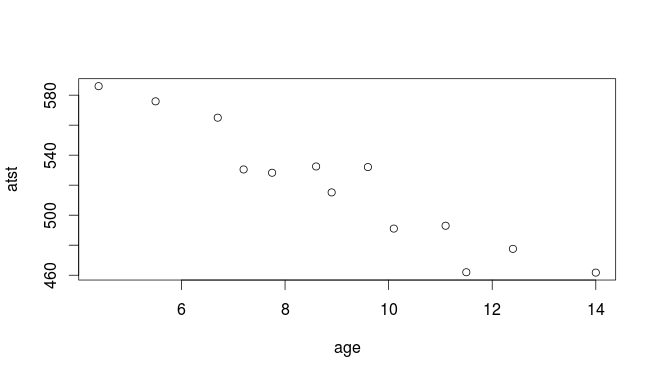
\includegraphics[width=\textwidth]{sleep-times}

\end{frame}

\begin{frame}[fragile]{The regression}

Scatterplot shows no obvious curve, and a pretty clear downward trend. So we can run the regression:

{\scriptsize
\begin{semiverbatim}
sleep.1=lm(atst~age)
summary(sleep.1)

Call:
lm(formula = atst ~ age)

Residuals:
    Min      1Q  Median      3Q     Max 
-23.011  -9.365   2.372   6.770  20.411 

Coefficients:
            Estimate Std. Error t value Pr(>|t|)    
(Intercept)  646.483     12.918   50.05 2.49e-14 ***
age          -14.041      1.368  -10.26 5.70e-07 ***
---
Signif. codes:  0 ‘***’ 0.001 ‘**’ 0.01 ‘*’ 0.05 ‘.’ 0.1 ‘ ’ 1 

Residual standard error: 13.15 on 11 degrees of freedom
Multiple R-squared: 0.9054,	Adjusted R-squared: 0.8968 
F-statistic: 105.3 on 1 and 11 DF,  p-value: 5.7e-07 
\end{semiverbatim}
}

\end{frame}

\begin{frame}{Conclusions}

    \begin{itemize}
  \item The relationship appears to be a straight line, with a downward trend.
  \item $F$-tests for model as a whole and $t$-test for slope (same) both confirm this.
  \item Slope is $-14$, so a 1-year increase in age goes with a 14-minute decrease in ATST on average.
  \end{itemize}
  
\end{frame}

% for week 2:
% 
% regression and multiple regression
% 
% including univariate + tests
% ci, pi and influential points
% multiple, re-interpretation of tests, correlated x's
% residuals and plotting
% 

% next: ci and pi with children aged 10 and 3
% then: maybe diagnostics

\begin{frame}{CI for mean response and prediction intervals}

Once useful regression exists, use it for prediction:


\begin{itemize}
\item To get a single number for prediction at a given $x$, substitute into regression equation, eg.\ age 10: predicted ATST is $646.48-14.04(10)=506$ minutes.
\item To express uncertainty of this prediction:
  \begin{itemize}
  \item {\em CI for mean response} expresses uncertainty about mean ATST for all children aged 10, based on data.
  \item {\em Prediction interval} expresses uncertainty about predicted ATST for a new child aged 10 whose ATST not known. More uncertain.
  \end{itemize}
\item Also do above for a child aged 3.
\end{itemize}
\end{frame}
\begin{frame}[fragile]{Intervals}
\begin{itemize}
\item Make new data frame with these values for \texttt{age}
\item Feed into \texttt{predict}
{\scriptsize
\begin{semiverbatim}
ages.new=data.frame(age=c(10,3))
ages.new
  age
1  10
2   3
pc=predict(sleep.1,ages.new,interval="c")
pp=predict(sleep.1,ages.new,interval="p")
cbind(ages.new,pc,pp)
  age      fit      lwr      upr      fit      lwr      upr
1  10 506.0729 497.5574 514.5883 506.0729 475.8982 536.2475
2   3 604.3602 584.4305 624.2899 604.3602 569.2149 639.5055  
\end{semiverbatim}
}
\end{itemize}

\end{frame}

\begin{frame}[fragile]{Comments}

\begin{itemize}
\item Age 10 closer to centre of data, so intervals are both narrower than those for age 3.
\item Age 3 assumes that straight line continues to hold (don't have any data to support that)
\item Prediction intervals bigger than CI for mean (additional uncertainty).
\end{itemize}

\end{frame}

\begin{frame}[fragile]{Diagnostics}
How do we tell whether a straight-line regression is appropriate?

\vspace{3ex}

\begin{itemize}
\item Before: check scatterplot for straight trend.
\item After: plot {\em residuals} (observed minus predicted response) against predicted values. Aim: a plot with no pattern.
\end{itemize}

\vspace{3ex}

\begin{verbatim}
plot(sleep.1)
\end{verbatim}

\end{frame}

\begin{frame}[fragile]{Output}

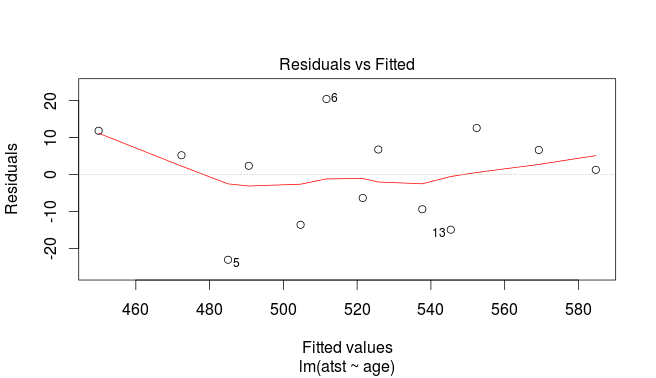
\includegraphics[width=4in]{sleep-resid}

Not much pattern here (is residual predictable from predicted? No). Good, indicating regression appropriate.
  
\end{frame}


\begin{frame}[fragile]{An inappropriate regression}

Scatterplot of different data:

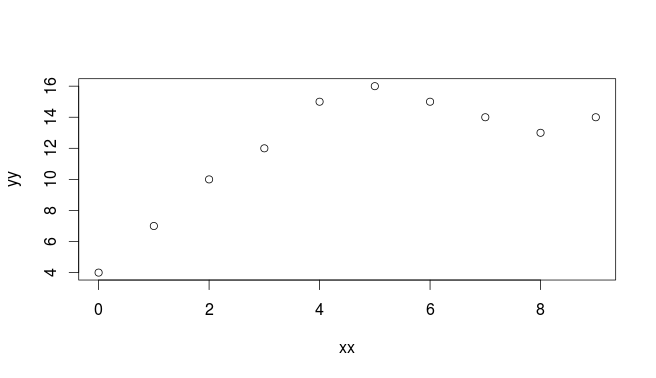
\includegraphics[width=4in]{curvy-scatter}

Trend goes up, then levels off, but a line would keep going up.

\end{frame}

\begin{frame}[fragile]{Regression line}

Try fitting a regression line anyway:

{\scriptsize
\begin{semiverbatim}
curvy=read.table("curvy.txt",header=T)
attach(curvy)
plot(xx,yy)
curvy.1=lm(yy~xx)
summary(curvy.1)
Call:
lm(formula = yy ~ xx)

Residuals:
   Min     1Q Median     3Q    Max 
-3.582 -2.204  0.000  1.514  3.509 

Coefficients:
            Estimate Std. Error t value Pr(>|t|)   
(Intercept)   7.5818     1.5616   4.855  0.00126 **
xx            0.9818     0.2925   3.356  0.00998 **
---
Signif. codes:  0 ‘***’ 0.001 ‘**’ 0.01 ‘*’ 0.05 ‘.’ 0.1 ‘ ’ 1 

Residual standard error: 2.657 on 8 degrees of freedom
Multiple R-squared: 0.5848,	Adjusted R-squared: 0.5329 
F-statistic: 11.27 on 1 and 8 DF,  p-value: 0.009984 

plot(curvy.1)
\end{semiverbatim}
}
  
\end{frame}



\begin{frame}[fragile]{Residual plot}

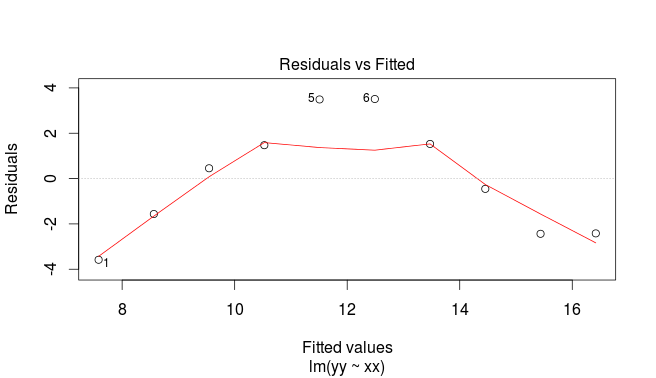
\includegraphics[width=4in]{curvy-residual}

Residual plot has {\em curve}: middle residuals positive, high and low ones negative. Bad.
  
\end{frame}

\begin{frame}[fragile]{Fixing it up}


\vspace{3ex}

Fitting a curve would be better. Try this:

{\scriptsize
\begin{semiverbatim}
xxsq=xx^2
curvy.2=lm(yy~xx+xxsq)
summary(curvy.2)

Call:
lm(formula = yy ~ xx + xxsq)
<...>
Coefficients:
            Estimate Std. Error t value Pr(>|t|)    
(Intercept)  3.90000    0.77312   5.045 0.001489 ** 
xx           3.74318    0.40006   9.357 3.31e-05 ***
xxsq        -0.30682    0.04279  -7.170 0.000182 ***
---
Signif. codes:  0 ‘***’ 0.001 ‘**’ 0.01 ‘*’ 0.05 ‘.’ 0.1 ‘ ’ 1 

Residual standard error: 0.9833 on 7 degrees of freedom
Multiple R-squared: 0.9502,	Adjusted R-squared: 0.936 
F-statistic: 66.83 on 2 and 7 DF,  p-value: 2.75e-05 
\end{semiverbatim}
}

\end{frame}


\begin{frame}{The residual plot now}

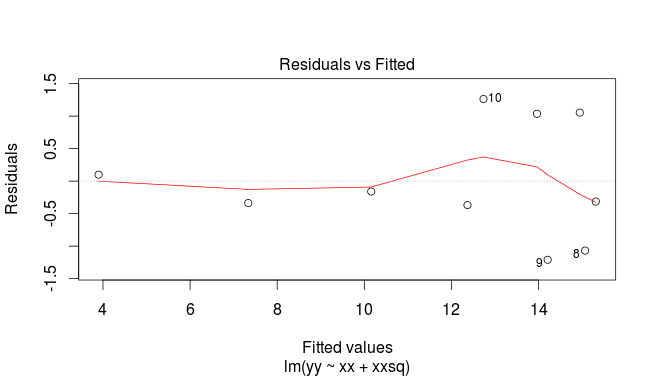
\includegraphics[width=4in]{curvy-resid2}

No problems any more.  

\end{frame}

%%%%%%%%%%%%%%%%%%%%%%%%%%%%%%%%%%%%%%%%%%%%

\begin{frame}[fragile]{Multiple regression}

  \begin{itemize}
  \item What if more than one $x$? Extra issues: % regression ex from before
    \begin{itemize}
    \item Now one intercept and a slope for each $x$: how to interpret?
    \item Which $x$-variables actually help to predict $y$?
 Different interpretations of ``global'' $F$-test and individual $t$-tests.
    \end{itemize}
  \item In \verb-lm- line, add extra $x$s after \verb-~-.
  \item Interpretation not so easy (and other problems that can occur).
  \end{itemize}

\end{frame}

\begin{frame}[fragile]{Multiple regression example}

Study of women and visits to health professionals, and how the number of visits might be related to other variables:

\begin{description}
\item[timedrs:] number of visits to health professionals (over course of study)
\item[phyheal:] number of physical health problems
\item[menheal:] number of mental health problems
\item[stress:] result of questionnaire about number and type of life changes
\end{description}

\verb-timedrs- response, others explanatory.

\end{frame}

\begin{frame}[fragile]{The code}


{\small
\begin{semiverbatim}
visits=read.table("regressx.txt",header=T)
head(visits)
attach(visits)
visits.1=lm(timedrs~phyheal+menheal+stress)
summary(visits.1)
\end{semiverbatim}
}

\end{frame}

\begin{frame}[fragile]{Output part 1}

{\scriptsize
\begin{semiverbatim}
Call:
lm(formula = timedrs ~ phyheal + menheal + stress)

Residuals:
    Min      1Q  Median      3Q     Max 
-14.792  -4.353  -1.815   0.902  65.886 

Coefficients:
             Estimate Std. Error t value Pr(>|t|)    
(Intercept) -3.704848   1.124195  -3.296 0.001058 ** 
phyheal      1.786948   0.221074   8.083  5.6e-15 ***
menheal     -0.009666   0.129029  -0.075 0.940318    
stress       0.013615   0.003612   3.769 0.000185 ***
---
Signif. codes:  0 ‘***’ 0.001 ‘**’ 0.01 ‘*’ 0.05 ‘.’ 0.1 ‘ ’ 1 

Residual standard error: 9.708 on 461 degrees of freedom
Multiple R-squared: 0.2188,	Adjusted R-squared: 0.2137 
F-statistic: 43.03 on 3 and 461 DF,  p-value: < 2.2e-16 

\end{semiverbatim}
}

\end{frame}


\begin{frame}[fragile]{The slopes}

Model as a whole strongly significant even though R-sq not very big (lots of data). At least one of the $x$'s predicts \verb-timedrs-.

(repeat output)

{\scriptsize
\begin{semiverbatim}
Coefficients:
             Estimate Std. Error t value Pr(>|t|)    
(Intercept) -3.704848   1.124195  -3.296 0.001058 ** 
phyheal      1.786948   0.221074   8.083  5.6e-15 ***
menheal     -0.009666   0.129029  -0.075 0.940318    
stress       0.013615   0.003612   3.769 0.000185 ***
---
Signif. codes:  0 ‘***’ 0.001 ‘**’ 0.01 ‘*’ 0.05 ‘.’ 0.1 ‘ ’ 1 

\end{semiverbatim}
}

The physical health and stress variables definitely help to predict the number of visits, but {\em with those in the model} we don't need \verb-menheal-.


However, look at prediction of \verb-timedrs- from \verb-menheal- by itself:
  
\end{frame}

\begin{frame}[fragile]{Just menheal}

{\scriptsize
\begin{semiverbatim}
> visits.2=lm(timedrs~menheal)
> summary(visits.2)

Call:
lm(formula = timedrs ~ menheal)
<...>
Coefficients:
            Estimate Std. Error t value Pr(>|t|)    
(Intercept)   3.8159     0.8702   4.385 1.44e-05 ***
menheal       0.6672     0.1173   5.688 2.28e-08 ***
---
Signif. codes:  0 ‘***’ 0.001 ‘**’ 0.01 ‘*’ 0.05 ‘.’ 0.1 ‘ ’ 1 

Residual standard error: 10.6 on 463 degrees of freedom
Multiple R-squared: 0.06532,	Adjusted R-squared: 0.0633 
F-statistic: 32.35 on 1 and 463 DF,  p-value: 2.279e-08 

\end{semiverbatim}
}

\verb-menheal- by itself {\em does} significantly help to predict \verb-timedrs-. But the R-sq is much less (6.5\% vs.\ 22\%) so the other two variables do a better job of prediction. 


\end{frame}

\begin{frame}[fragile]{Residual plot}


Go back to regression of \verb-timedrs- on all $x$'s: predicts significantly, but is it appropriate? Look at plot of residuals vs.\ predicted values.


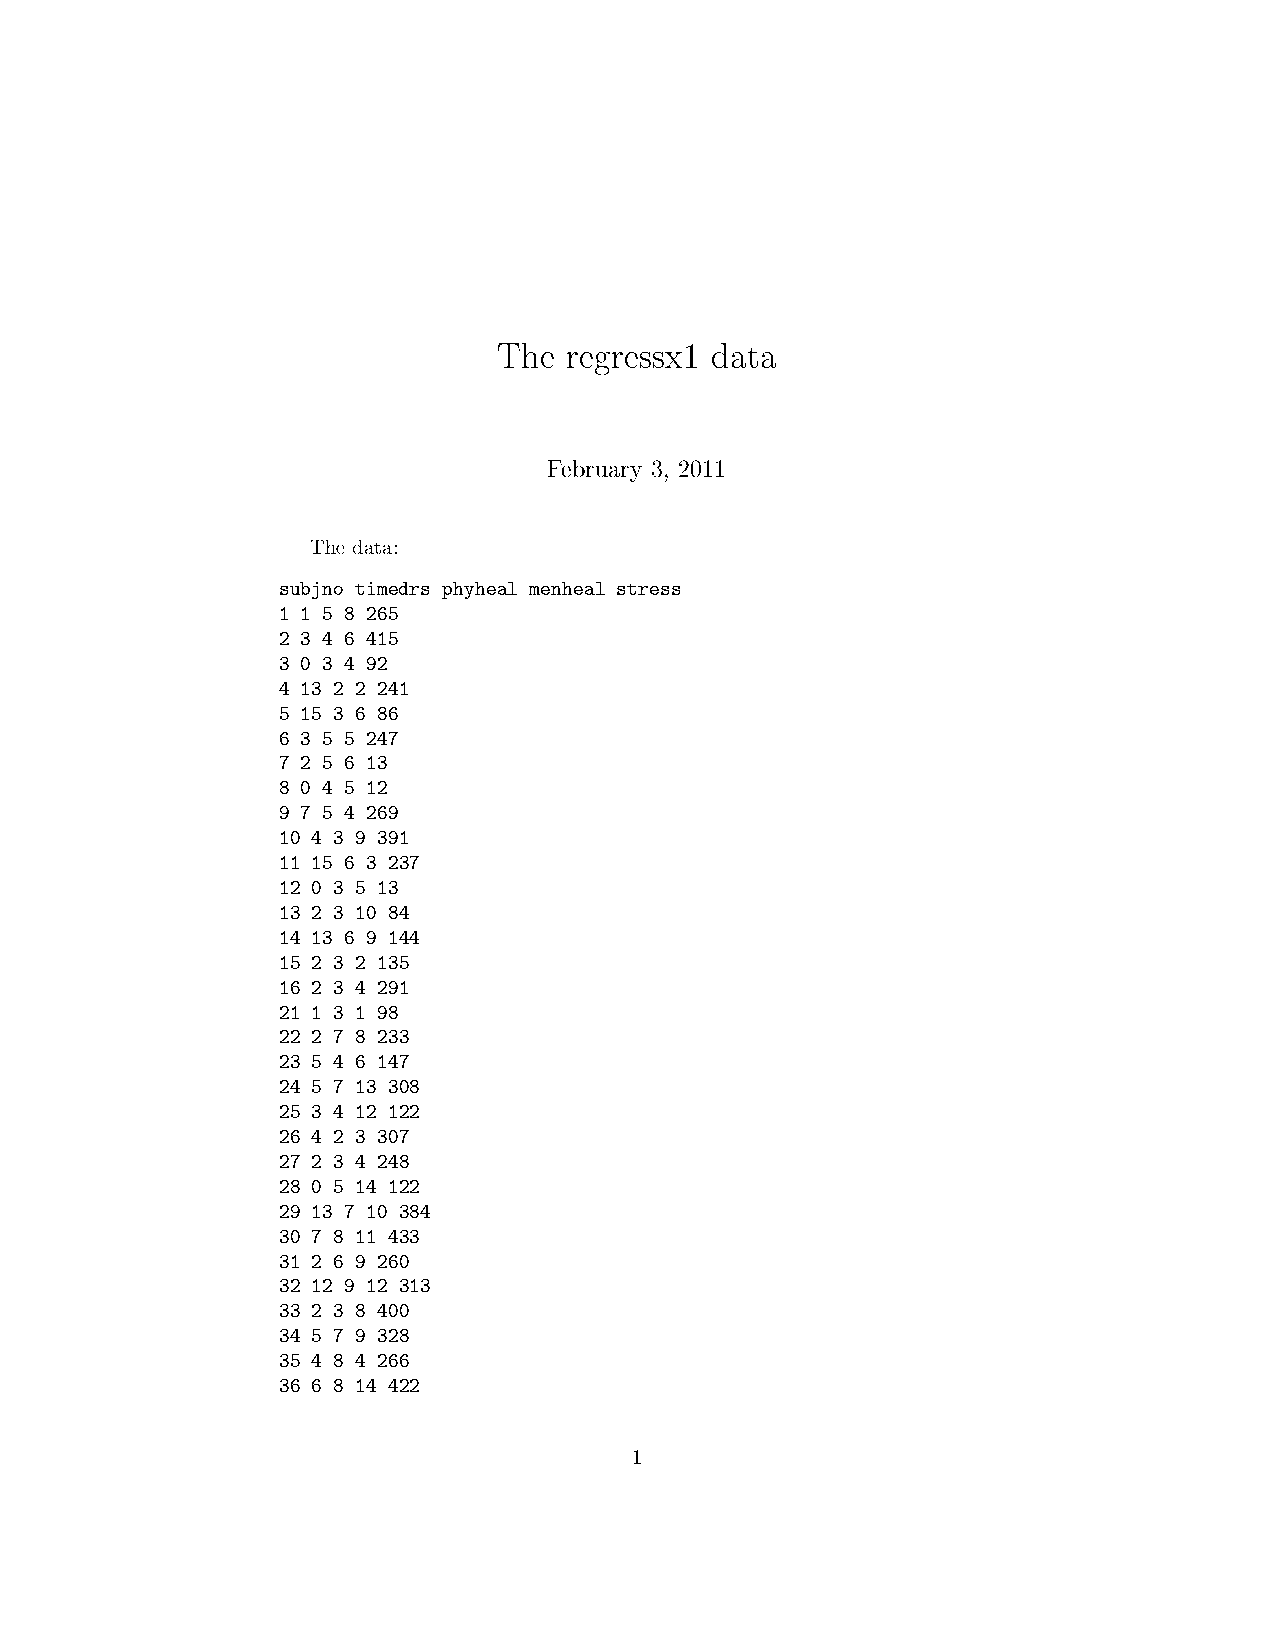
\includegraphics[width=4in]{regressx1}

\end{frame}

\begin{frame}[fragile]{Normal QQ plot of residuals}

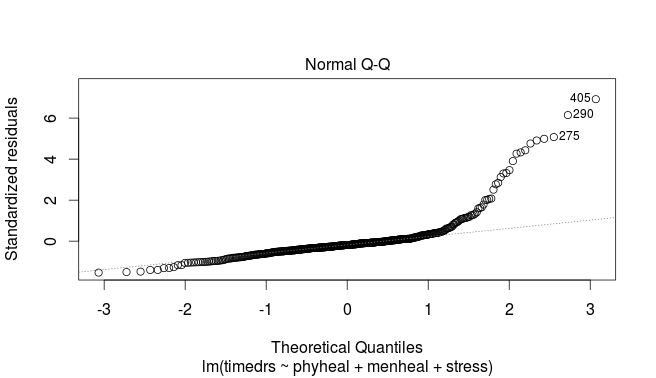
\includegraphics[width=\textwidth]{regressx1a}
  
\end{frame}

\begin{frame}{Residuals are not normal}

  \begin{itemize}
  \item No pattern
  \item but some very positive residuals (compared to
how negative).
\item Distribution of residuals is {\em skewed}, not
normal as it should be.
  \end{itemize}
\end{frame}


\begin{frame}[fragile]{Fixing the problems}

  \begin{itemize}
  \item Sometimes residuals are {\em very} positive: observed a {\em lot} larger than predicted.
  \item Try {\em  transforming} response: use log or square root of response. (Note that response is {\em count}, often skewed to right.)
  \item Try regression again. Define transformed \verb-timedrs- in data step, and use transformed variable as response. Check residual plot to see that it is OK now:

{\footnotesize
\begin{semiverbatim}
lgtime=log(timedrs+1)
visits.3=lm(lgtime~phyheal+menheal+stress)
plot(visits.3)
\end{semiverbatim}
}
  \end{itemize}
  
\end{frame}


\begin{frame}[fragile]{Output}
  
{\scriptsize
\begin{semiverbatim}
> summary(visits.3)

Call:
lm(formula = lgtime ~ phyheal + menheal + stress)

Residuals:
     Min       1Q   Median       3Q      Max 
-1.95865 -0.44076 -0.02331  0.42304  2.36797 

Coefficients:
             Estimate Std. Error t value Pr(>|t|)    
(Intercept) 0.3903862  0.0882908   4.422 1.22e-05 ***
phyheal     0.2019361  0.0173624  11.631  < 2e-16 ***
menheal     0.0071442  0.0101335   0.705    0.481    
stress      0.0013158  0.0002837   4.638 4.58e-06 ***
---
Signif. codes:  0 ‘***’ 0.001 ‘**’ 0.01 ‘*’ 0.05 ‘.’ 0.1 ‘ ’ 1 

Residual standard error: 0.7625 on 461 degrees of freedom
Multiple R-squared: 0.3682,	Adjusted R-squared: 0.3641 
F-statistic: 89.56 on 3 and 461 DF,  p-value: < 2.2e-16 

\end{semiverbatim}
}

\end{frame}

\begin{frame}[fragile]{Comments}

  \begin{itemize}
  \item Model as a whole strongly significant again 
  \item R-sq higher than before (37\% vs.\ 22\%) suggesting things more linear now
  \item Same conclusion re \verb-menheal-: can take out of regression.
  \item Should look at residual plot (next page).
  \end{itemize}
  
\end{frame}

\begin{frame}[fragile]{The residual plot}

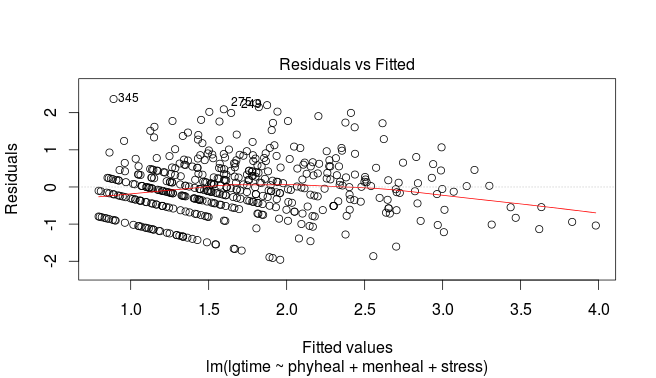
\includegraphics[width=4in]{regressx2}

Much better. Residuals range from 2 to $-2$, and look symmetric in shape. Should be trustworthy now.
  
\end{frame}

\begin{frame}[fragile]{Normal QQ plot of residuals}

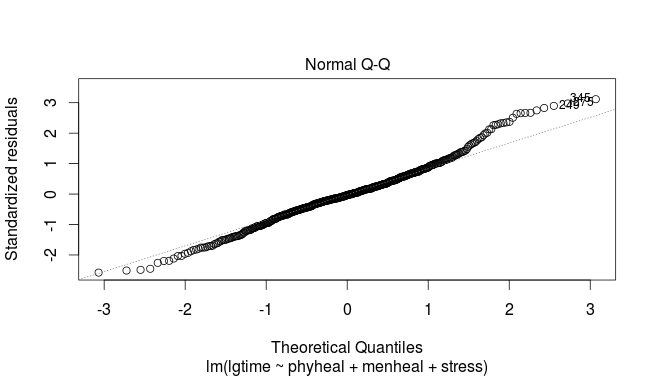
\includegraphics[width=4in]{regressx2a}

  
\end{frame}

\begin{frame}[fragile]{Box-Cox transformations}


  \begin{itemize}
  \item Taking log of \verb-timedrs- and having it work: lucky
    guess. How to find good transformation?
  \item Idea: Box-Cox: {\em estimate} the kind of transformation that
    would work: take power of response (1 = no change, 0.5 = square
    root, {\em 0 = log}).
  \item \texttt{boxcox} in package \texttt{MASS}.
  \end{itemize}

\end{frame}

\begin{frame}[fragile]{\texttt{boxcox}}
  \begin{itemize}
  \item Some of \verb-timedrs- values are 0, but Box-Cox expects all
    +. Define new variable \verb-tp- in data step, then call
    \verb-boxcox- with that as response.

\begin{verbatim}
tp=timedrs+1
library(MASS)
boxcox(tp~phyheal+menheal+stress)
\end{verbatim}


  \item \verb-tp- only necessary here because of zeros in
    \verb-timedrs-; normally omit and use original response in
    \verb-boxcox-.
  \item Output from \texttt{boxcox} is plot, as on next page.

\end{itemize}

\end{frame}

\begin{frame}[fragile]{Try 1}

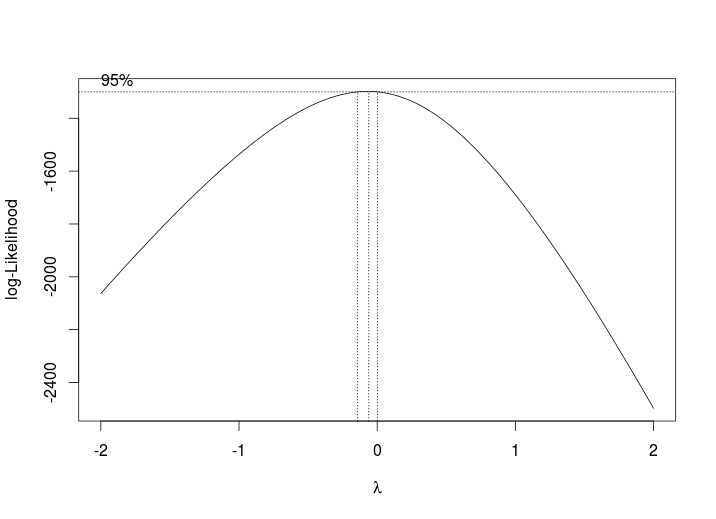
\includegraphics[width=0.8\textwidth]{boxcox}
\begin{itemize}
\item Best: $\lambda$ just less than zero.
\item Hard to see scale. 
\item Focus on $\lambda$ in $(-0.3,0.1)$.

\end{itemize}

\end{frame}


\begin{frame}[fragile]{Try 2}

{\footnotesize
  \begin{semiverbatim}
boxcox(tp~phyheal+menheal+stress,lambda=seq(-0.3,0.1,0.01))
    \end{semiverbatim}
}
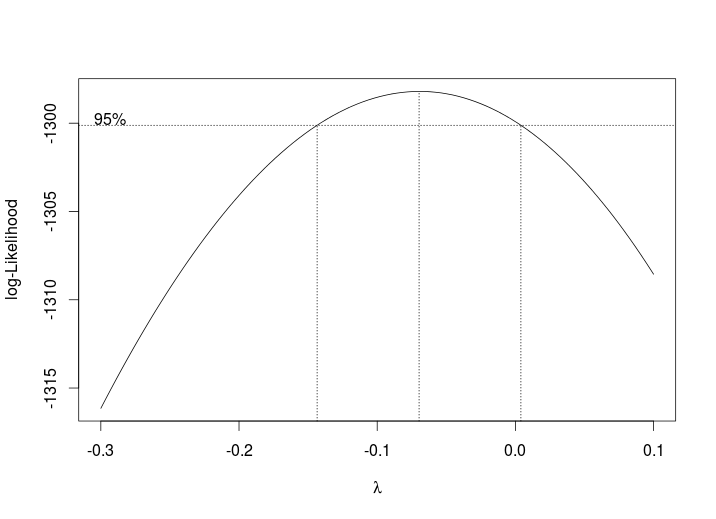
\includegraphics[width=0.7\textwidth]{boxcox2}
\begin{itemize}
\item Best: $\lambda$ just about $-0.07$.
\item CI for $\lambda$ about $(-0.14,0.01)$.
\item Only round number: $\lambda=0$, log transformation.
\end{itemize}

\end{frame}



\begin{frame}[fragile]{Testing more than one $x$ at once}

The $t$-tests test only whether one variable could be taken out of the
regression you're looking at. To test significance of more than one
variable at once, fit model with and without variables and use
\texttt{anova} to compare fit of models:

{\small
\begin{semiverbatim}
> visits.5=lm(lgtime~phyheal+menheal+stress)
> visits.6=lm(lgtime~stress)
> anova(visits.6,visits.5)
Analysis of Variance Table

Model 1: lgtime ~ stress
Model 2: lgtime ~ phyheal + menheal + stress
  Res.Df    RSS Df Sum of Sq      F    Pr(>F)    
1    463 371.47                                  
2    461 268.01  2    103.46 88.984 < 2.2e-16 ***
---
Signif. codes:  0 ‘***’ 0.001 ‘**’ 0.01 ‘*’ 0.05 ‘.’ 0.1 ‘ ’ 1 
\end{semiverbatim}
}

\end{frame}

\begin{frame}[fragile]{Results of tests}


\begin{itemize}
\item Test says ``taking both variables out makes the fit worse, so don't do it''.
\item There is significant difference between the two models, meaning
  the model with \emph{more} $x$'s fits better. Taking out those $x$'s
  is a mistake. Or putting them in is a good idea.
\end{itemize}
  
\end{frame}

\begin{frame}[fragile]{The punting data}

  Data set \verb-punting.dat- contains 4 variables for 13 right-footed
  football kickers (punters): left leg and right leg strength (lbs),
  distance punted (ft), another variable called ``fred''. Predict
  punting distance from other variables:

\begin{semiverbatim}
punting=read.table("punting.txt",header=T)
attach(punting)
punting.1=lm(punt~left+right+fred)
summary(punting.1)
\end{semiverbatim}

  
\end{frame}

\begin{frame}[fragile]{Regression output (edited)}
  
{\scriptsize
\begin{semiverbatim}
> punting.1=lm(punt~left+right+fred)
> summary(punting.1)

Call:
lm(formula = punt ~ left + right + fred)
<...>
Coefficients:
            Estimate Std. Error t value Pr(>|t|)
(Intercept)  -4.6855    29.1172  -0.161    0.876
left          0.2679     2.1111   0.127    0.902
right         1.0524     2.1477   0.490    0.636
fred         -0.2672     4.2266  -0.063    0.951

Residual standard error: 14.68 on 9 degrees of freedom
Multiple R-squared: 0.7781,	Adjusted R-squared: 0.7042 
F-statistic: 10.52 on 3 and 9 DF,  p-value: 0.00267 
\end{semiverbatim}
}

\end{frame}


\begin{frame}{Comments}

  \begin{itemize}
  \item Overall regression strongly significant, R-sq high.
  \item None of the $x$'s significant! Why?
  \item $t$-tests only say that you could take any one of the $x$'s out without damaging the fit; doesn't matter which one.
  \item Explanation: look at {\em correlations}. 
  \end{itemize}
\end{frame}

\begin{frame}[fragile]{The correlations}  


{\scriptsize
\begin{semiverbatim}
> cor(punting)
           left     right      punt      fred
left  1.0000000 0.8957224 0.8117368 0.9722632
right 0.8957224 1.0000000 0.8805469 0.9728784
punt  0.8117368 0.8805469 1.0000000 0.8679507
fred  0.9722632 0.9728784 0.8679507 1.0000000
\end{semiverbatim}
}

{\em All} correlations are high: $x$'s with \verb-punt- (good) and
with each other (bad, at least confusing).

What to do? Probably do just as well to pick one variable, say
\texttt{right} since kickers are right-footed.

\end{frame}

\begin{frame}[fragile]{Just \texttt{right}}

{\scriptsize
\begin{semiverbatim}
> punting.2=lm(punt~right)
> anova(punting.2,punting.1)
Analysis of Variance Table

Model 1: punt ~ right
Model 2: punt ~ left + right + fred
  Res.Df    RSS Df Sum of Sq      F Pr(>F)
1     11 1962.5                           
2      9 1938.2  2    24.263 0.0563 0.9456
\end{semiverbatim}
}

No significant loss by dropping other two variables.
Compare R-squareds for the two models:

{\scriptsize
  \begin{semiverbatim}
> summary(punting.1)$r.squared
[1] 0.7781401
> summary(punting.2)$r.squared
[1] 0.7753629    
  \end{semiverbatim}
}

Basically no difference.
  
\end{frame}

\begin{frame}[fragile]{Regression results}
  
{\scriptsize
  \begin{semiverbatim}
> summary(punting.2)

Call:
lm(formula = punt ~ right)

Residuals:
     Min       1Q   Median       3Q      Max 
-15.7576 -11.0611   0.3656   7.8890  19.0423 

Coefficients:
            Estimate Std. Error t value Pr(>|t|)    
(Intercept)  -3.6930    25.2649  -0.146    0.886    
right         1.0427     0.1692   6.162 7.09e-05 ***
---
Signif. codes:  0 ‘***’ 0.001 ‘**’ 0.01 ‘*’ 0.05 ‘.’ 0.1 ‘ ’ 1 

Residual standard error: 13.36 on 11 degrees of freedom
Multiple R-squared: 0.7754,	Adjusted R-squared: 0.7549 
F-statistic: 37.97 on 1 and 11 DF,  p-value: 7.088e-05 
    
  \end{semiverbatim}
}
\end{frame}

